\section{Camera module testing}

The camera module and controller were tested throughout their development and thus problems were quickly discovered and swiftly rectified.

\subsection{Existing Software}

The uCam has a freely downloadable piece of software that allows you to test the uCam and verify its functions. If you can connect the uCam to a COM port on the computer then you can sync with it and then take and view pictures in the different available formats and resolutions.

This allowed for not just the functionality of the camera to be verified but said functionality was then compared to the specification and it was shown that the uCam should be able to provide what is required from the camera module.

[] image taken from camera with software []

\subsection{Arduino Implementation}

With the camera communication and SD-card successfully implemented it could be readily shown that a picture could be taken and stored. These photos could then be viewed on the computer.

\begin{figure}[H]
        \centering
        \includegraphics[width=1.00\textwidth]{figures/nyanNyan.jpg}
        \captionof{figure}{Test image captured using the arduino implementation of the camera controller}
        \label{fig:Nyan1}
\end{figure}

The testing during development means that functionality of the controller has been verified already, the test that needs to be performed on this element of the system is to time how long it takes to get an image from the camera and save it to the SD-card and check that this is well within the 3 minutes allowed by the specification. Timing of this process showed that it took around 5 seconds to complete, so well within the 3 minute limit in the specification.

\subsection{Integrated Implementation}

During the integration process the system was regularly tested for functionality and any errors were fixed as the system was developed. A large number of images were taken during this process and during the implementation of additional features.

\begin{figure}[H]
        \centering
        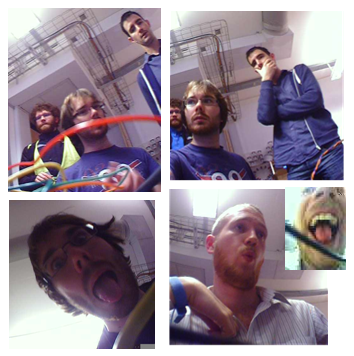
\includegraphics[width=1.00\textwidth]{figures/SampleImages1.png}
        \captionof{figure}{Test images captured using the integrated implementation of the camera controller}
        \label{fig:Samples1}
\end{figure}

The system can capture images at the 640x480 resolution specified and can also capture images at the other resolutions at which the uCam will take jpeg images. Currently the option to capture raw images is not implemented.

The time taken for the system to capture an image at maximum resolution, save it to SD-card and then download and display it on the ground station software was measured at around 10 to 15 seconds |||||| TRIPLE CHECK |||||||. This is still well within the 3 minutes specified and has large amounts of overhead meaning that it should remain well within that limit even if there are other payloads implemented on the UAV or if a lot of packets are dropped and have to be resent.